%%%%%%%%%%%%%%%%%%%%%%%%%%%%%%%%%%%%%%%%%%%%%%%%%%%%%%%%%%%%%%%%%%%%%%%%%%%%%%%%
% File: memoria.tex
% Created: 2011-11-11-12:55 by Leo Ferres
% Modified:
% 2011-11-11-12:55 by Leo Ferres
%
% This is a LaTeX file intended to serve as the boilerplate code for
% "memorias", masters and PhD thesis in the Department of Computer
% Science at the Universidad de Concepción. The idea is to also
% include information relevant for students, such as tips on the
% document, and generally knowledge about how to write these kinds of
% documents, so check http://www.inf.udec.cl/~leo/fdoc.tex.
%%%%%%%%%%%%%%%%%%%%%%%%%%%%%%%%%%%%%%%%%%%%%%%%%%%%%%%%%%%%%%%%%%%%%%%%%%%%%%%%
\documentclass[12pt]{diicc}

%%%%%%%%%%%%%%%%%%%%%%%%%%%%%%%%%%%%%%%%%%%%%%%%%%%%%%%%%%%%%%%%%%%%%%%%%%%%%%%%
% Step 1: Add your packages here
%
% http://math.kangwon.ac.kr/~yhpark/tex/packages.html
%%%%%%%%%%%%%%%%%%%%%%%%%%%%%%%%%%%%%%%%%%%%%%%%%%%%%%%%%%%%%%%%%%%%%%%%%%%%%%%%
\usepackage{setspace}
\usepackage{graphicx}
\setcounter{secnumdepth}{3}
\usepackage[linesnumbered,ruled,vlined]{algorithm2e}
\usepackage{url}
\usepackage{amsmath, amsthm, amssymb}
\usepackage{mathtools}


%%%%%%%%%%%%%%%%%%%%%%%%%%%%%%%%%%%%%%%%%%%%%%%%%%%%%%%%%%%%%%%%%%%%%%%%%%%%%%%%
% Step 2: Un-comment these commands if this is a draft
%
%%%%%%%%%%%%%%%%%%%%%%%%%%%%%%%%%%%%%%%%%%%%%%%%%%%%%%%%%%%%%%%%%%%%%%%%%%%%%%%%
%\draft
%\singlespace

%%%%%%%%%%%%%%%%%%%%%%%%%%%%%%%%%%%%%%%%%%%%%%%%%%%%%%%%%%%%%%%%%%%%%%%%%%%%%%%%
% Step 3: Add your definitions here
%
% http://en.wikibooks.org/wiki/LaTeX/Customizing_LaTeX
%%%%%%%%%%%%%%%%%%%%%%%%%%%%%%%%%%%%%%%%%%%%%%%%%%%%%%%%%%%%%%%%%%%%%%%%%%%%%%%%
\newcommand{\ignore}[1]{}

%%%%%%%%%%%%%%%%%%%%%%%%%%%%%%%%%%%%%%%%%%%%%%%%%%%%%%%%%%%%%%%%%%%%%%%%%%%%%%%%
% Step 4: Choose your degree
% You can write either \eng for Engineering, \msc for Masters and \phd
% for Doctor of Philosophy. Engineering is set as default.
%%%%%%%%%%%%%%%%%%%%%%%%%%%%%%%%%%%%%%%%%%%%%%%%%%%%%%%%%%%%%%%%%%%%%%%%%%%%%%%%
\eng

%%%%%%%%%%%%%%%%%%%%%%%%%%%%%%%%%%%%%%%%%%%%%%%%%%%%%%%%%%%%%%%%%%%%%%%%%%%%%%%%
% Step 5: Choose title and add author
%%%%%%%%%%%%%%%%%%%%%%%%%%%%%%%%%%%%%%%%%%%%%%%%%%%%%%%%%%%%%%%%%%%%%%%%%%%%%%%%
\title{\bf Physical sharing of clauses in parallel SAT solvers}
\author{Juan Luis Olate Hinrichs}

%%%%%%%%%%%%%%%%%%%%%%%%%%%%%%%%%%%%%%%%%%%%%%%%%%%%%%%%%%%%%%%%%%%%%%%%%%%%%%%%
% Step 6: Add your advisor
%%%%%%%%%%%%%%%%%%%%%%%%%%%%%%%%%%%%%%%%%%%%%%%%%%%%%%%%%%%%%%%%%%%%%%%%%%%%%%%%
\advisor{Leo Ferres}

%%%%%%%%%%%%%%%%%%%%%%%%%%%%%%%%%%%%%%%%%%%%%%%%%%%%%%%%%%%%%%%%%%%%%%%%%%%%%%%%
% Step 7: Set your submission, copyright and defense dates. 
%
% Notice that these are not typeset. But they do serve a purpose for
% future references.
%%%%%%%%%%%%%%%%%%%%%%%%%%%%%%%%%%%%%%%%%%%%%%%%%%%%%%%%%%%%%%%%%%%%%%%%%%%%%%%%
\submitdate{September, 2011} % date you submitted to the committee
\defensedate{Octubre, 2011}  % date the defense was set
\copyrightyear{2011}         % document for final archiving

\begin{document}
\frontmatter

%%%%%%%%%%%%%%%%%%%%%%%%%%%%%%%%%%%%%%%%%%%%%%%%%%%%%%%%%%%%%%%%%%%%%%%%%%%%%%%%
% Step 8: Acknowledgments and dedication
%
% Uncomment this in the final version
%%%%%%%%%%%%%%%%%%%%%%%%%%%%%%%%%%%%%%%%%%%%%%%%%%%%%%%%%%%%%%%%%%%%%%%%%%%%%%%%
% \begin{acknowledgements}
% .....
% \end{acknowledgements}

% \begin{dedication}
% To my parents, my family, and whomever it may concern...  
% \end{dedication}

%%%%%%%%%%%%%%%%%%%%%%%%%%%%%%%%%%%%%%%%%%%%%%%%%%%%%%%%%%%%%%%%%%%%%%%%%%%%%%%%
% Step 9: Add abstract
%
% http://research.berkeley.edu/ucday/abstract.html
%%%%%%%%%%%%%%%%%%%%%%%%%%%%%%%%%%%%%%%%%%%%%%%%%%%%%%%%%%%%%%%%%%%%%%%%%%%%%%%%
\begin{abstract}
Your abstract goes here...
\end{abstract}

%%%%%%%%%%%%%%%%%%%%%%%%%%%%%%%%%%%%%%%%%%%%%%%%%%%%%%%%%%%%%%%%%%%%%%%%%%%%%%%%
% Step 10: Add an introduction
%
% 
%%%%%%%%%%%%%%%%%%%%%%%%%%%%%%%%%%%%%%%%%%%%%%%%%%%%%%%%%%%%%%%%%%%%%%%%%%%%%%%%
\mainmatter
\chapter{Introduction}\label{chap:intro}

One of the most well-known problems in computer \cite{drepper2007} science is the satisfiability (SAT) problem. This is because this was the first problem to be proved to be NP-complete \cite{cook1971}, proof known as the Cook-Levin theorem\footnote[1]{They both proved it independently.}. One year later, in 1972, Karp proved in \cite{karp1972} that many common combinatorial problems could be reduced in polynomial time to instances of the SAT problem, thus drawing even more attention to SAT problems by the scientific community. Because many combinatorial problems can be reduced to SAT, it is not strange to find many practical problems with useful applications (such as circuit design and automatic theorem proving) that could be solved if there was an efficient algorithm to solve the SAT problem. Unfortunately, because of the NP-complete nature of SAT, such algorithm has not been found yet, but also has not been proven to be in-existent. Many researchers suspect such efficient algorithm to solve all SAT instances does not exist, so instead of trying to solve the NP-complete problem, they try to improve the current SAT solving algorithms.Over the years, SAT solvers have shown impressive improvement, the first complete algorithm, the Davis Putnam algorithm \cite{DP1960}, was very limited and could only handle problems with around ten variables. Today, modern SAT solvers can handle instances with millions of variables, making such solvers suitable even for industrial application. In the next chapter we will point out the main features that have improved SAT solvers significantly. 

In the last decade parallel computing has become increasingly popular. As CPU manufacturers have found difficult and expensive to keep increasing the clock speed of processors, they have instead turn to increase the number of cores each chip has. Unfortunately, if the algorithms are not thought to be run in parallel, more cores will bring small improvements. This is the reason why there is a growing concern to parallelize algorithms so that they can take advantage of many-cores architectures of today's computers. In SAT solving it is no different. The annual SAT competition \footnote[1]{www.satcompetition.org}, an event to determine which is the fastest SAT solver, has two main categories; sequential SAT solvers and parallel SAT solvers. In the last years parallel SAT solvers have outperformed sequential solvers in total wall clock time, so the interest in parallel solvers has grown, new designs and approaches have been explored for this kind of solvers. One of the most successful approaches to implement a parallel SAT solver is the portfolio approach. This approach is basically to run different solvers in parallel and wait for one of them to solve the problem. It's a very simple and straight forward approach of parallelization, but we have also encountered one drawback to it: as we add more solvers to different cores of a single chip, the overall performance of the parallel solver decreases in around 20-40\%. In this work we will attempt to find the source of this problem and explore possible solutions to it. 




%%%%%%%%%%%%%%%%%%%%%%%%%%%%%%%%%%%%%%%%%%%%%%%%%%%%%%%%%%%%%%%%%%%%%%%%%%%%%%%%
% Step 11: Add background and literature review
%
% 
%%%%%%%%%%%%%%%%%%%%%%%%%%%%%%%%%%%%%%%%%%%%%%%%%%%%%%%%%%%%%%%%%%%%%%%%%%%%%%%%
\chapter{Background and Related Work}\label{chap:background}
\section{SAT solvers}

\subsection{The SAT problem}

Given a set of boolean variables $\Sigma$, a literal $L$ is either a variable or the negation of a variable in $\Sigma$, and a \textit{clause} is a disjunction of literals over distinct variables\footnote[1]{That all literals in a clause have to be over distinct variables is not standard.}. A propositional sentence is in \textit{conjunctive normal form} (\textit{CNF}) if it has the form $\alpha_{1} \wedge \alpha_{2} \wedge ... \wedge \alpha_{n}$, where each $\alpha_{i}$ is a clause. The notation of sentences in CNF we will be using are sets. A clause $l_{1} \vee l_{2} \vee ... \vee l_{m}$, where $l_{i}$ is a literal, can be expressed as the set $\{l_{1},l_{2},...,l_{m}\}$. Furthermore, the CNF $\alpha_{1} \wedge \alpha_{2} \wedge ... \wedge \alpha_{n}$ can be expressed as the set of clauses $\{\alpha_{1},\alpha_{2},...,\alpha_{n}\}$. With these conventions, a CNF $\Delta$ is valid if $\Delta$ is the empty set: $\Delta = \emptyset$. A CNF $\Delta$ will be inconsistent if it contains the empty set: $\emptyset \in \Delta$. 
Given a CNF $\Delta$, the SAT problem is answering the question: Is there an assignment of values for variables in $\Sigma$, such that $\Delta$ evaluates to true? The NP-completeness of this question lies in the combinatorial nature of the problem; to solve it one would need to try all different assignments of variables in $\Sigma$, the number of possible assignments grows exponentially as $|\Sigma|$ grows.

\subsection{Resolution}
The resolution inference rule \cite{Rob65} is defined as follows. Let $P$ be a Boolean variable, and suppose that $\Delta$ is a CNF which contains clauses $C_{i}$ and $C_{j}$, where $P \in C_{i}$ and $\neg P \in C_{j}$. The resolution inference rule allows us to derive the clause $(C_{i}-\{P\})\cup (C_{j}-\{\neg P\})$, which is called a \textit{resolvent} that is obtained by \textit{resolving} $C_{i}$ and $C_{j}$. A simple example is the CNF $\{\{A,\neg B\},\{B,C\}\}$. Applying resolution to this two clauses would derive the clause $\{A,C\}$, which would be called a B-\textit{resolvent}.
Resolution is incomplete in the sense that it is not guaranteed to derive every clause that is implied by the CNF, but it is \textit{refutation complete} on CNFs. It is guaranteed that resolution will derive the empty clause if the given CNF is unsatisfiable. 

\textit{Unit resolution} is an important special case of resolution. It's a resolution strategy which requires that at least one of the resolved clauses has only one literal. Such clause is called a \textit{unit clause}. The importance of unit resolution does not rely on its completeness (it's actually not refutation complete, as resolution is), but one can apply all possible unit resolution steps in time linear to the size of a given CNF. Its efficiency makes it a key technique employed by modern solvers.

\subsection{Conditioning}
\textit{Conditioning} a CNF $\Delta$ on a literal $L$ consists of replacing every occurrence of $L$ by the constant \textbf{true}, replacing $\neg L$ with \textbf{false}, and simplifying accordingly. The result of conditioning $\Delta$ on $L$ will be denoted by $\Delta |L$ and can be defined as follows:
\[ \Delta |L=\{\alpha -\{\neg L\}|\alpha \in \Delta, L\notin \alpha\}\]
This means that the new set of clauses $\Delta |L$ will be all the clauses in $\Delta$ that do not contain $L$, but with the literal $\neg L$ removed. The clauses that contain $L$ are removed because they are now satisfied, since we made $L$ \textbf{true}. $\neg L$ is removed from the remaining clauses because it was set to \textbf{false} and no longer has any effect.

The definition of conditioning can be extended to multiple literals. For example, the CNF:
\[\Delta=\{\{A,B,\neg C\},\{\neg A,D\},\{B,C,D\}\}\]
can be conditioned as $\Delta |CA\neg D=\{\emptyset \}$ (an inconsistent CNF). Moreover, $\Delta |\neg CD=\emptyset$ (a valid CNF).

\subsection{Satisfiability by search: The DPLL algorithm.}

\subsubsection{Search trees}
One way to picture the search for a possible assignment of variables that satisfies the CNF formula is to use a tree. For example, given $\Sigma =\{A,B,C\}$ and $\Delta =\{\{\neg A,B\},\{\neg B,C\}\}$, figure ~\ref{fig:searchtree} shows the search tree for this CNF. Each node of the tree represents a variable, for each level we have a different variable. The branches are the different truth values the variable can be assigned. Each $w_{i}$ represents a possible truth assignment of the variables in $\Sigma$. Note that $w_{1}$, $w_{5}$, $w_{7}$ and $w_{8}$ are all assignments that satisfy the CNF, while $w_{2}$, $w_{3}$, $w_{4}$ and $w_{6}$ do not.

\begin{figure}[h!]
	\centering
		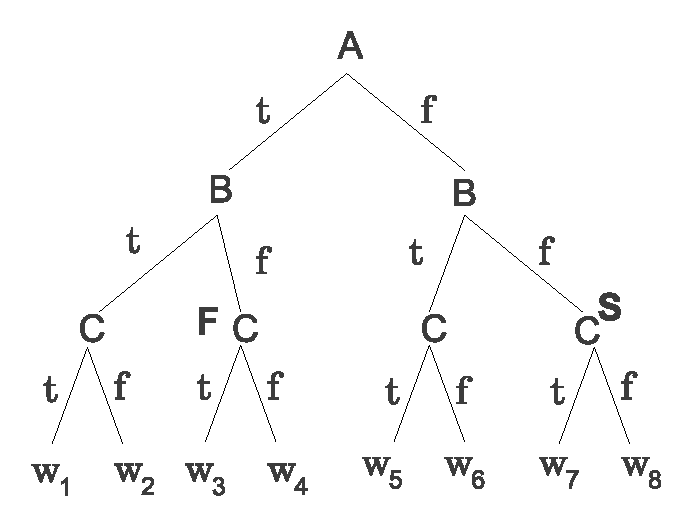
\includegraphics[width=0.5\textwidth]{searchtree}
	\caption{A search tree for the CNF $\Delta =\{\{\neg A,B\},\{\neg B,C\}\}$.}
	\label{fig:searchtree}
\end{figure}

\subsubsection{Depth-search-first algorithm}

\begin{algorithm}
\textsc{Depth-first-search}(CNF $\Delta$,depth $d$):\\
\uIf{$\Delta=\{\}$}{
	\bf{return \{\}}.
}
\uElseIf{$\{\}\in \Delta$}{
	\textbf{return} \textsc{unsatisfiable}
}
\uElseIf{\textsc{\textbf{L}}$=$\textsc{Depth-first-search}$(\Delta |P_{d+1},d+1)\neq$\textsc{unsatisfiable}}{
	\textbf{return} \textbf{L} $\cup$ $\{P_{d+1}\}$
}
\uElseIf{\textsc{\textbf{L}}$=$\textsc{Depth-first-search}$(\neg \Delta |P_{d+1},d+1)\neq$\textsc{unsatisfiable}}{
	\textbf{return} \textbf{L} $\cup$ $\{\neg P_{d+1}\}$
}
\Else{\textbf{return} \textsc{unsatisfiable}}
\caption{Depth-first-search algorithm\label{dpll}}
\end{algorithm}    

The Davis-Putnam-Logemann-Loveland (DPLL) \cite{dpll} algorithm is the base of all modern SAT solvers. Many refinements have been made to this algorithm over the last decade, which have been significant enough to change the behaviour of the algorithm, but it is still important to know it for understanding modern solvers. Figure ~\ref{fig:searchtree} shows a search tree with three variables. We can observe that the leaves of this tree and in one-to-one correspondence with all the possible true assignments of variables involved, so testing satisfiability can be viewed as searching for a leaf node that satisfies the CNF. Another important observation is that the depth of the tree is $n$, where $n$ is the number of boolean variables, so performing a depth-first-search would be best to explore the tree. Algorithm ~\ref{dpll} performs a depth-first-search, which is the base of the DPLL algorithm, using the conditioning operator on CNFs to remove clauses or reduce their size.

Consider the CNF:
\[\Delta=\{\{\neg A,B\},\{\neg B,C\}\},\]
and the search node labelled with \textbf{F} in Figure ~\ref{fig:searchtree}. At this node, Algorithm ~\ref{dpll} will condition $\Delta$ on literals $A,\neg B$, leading to:
\[\Delta |A,\neg B=\{ \{\textbf{false},\textbf{false}\},\{\textbf{true},C\}\}=\{\{\}\}.\]
The algorithm will detect that at this internal node that there is a contradiction, hence concluding that neither $w3$ or $w4$ are models of $\Delta$, without having to visit them explicitly. The algorithm can also detect success at internal nodes, implying that all assignments from that particular node are models of the CNF.

\subsubsection{Unit Resolution}

\begin{figure}[h!]
	\centering
		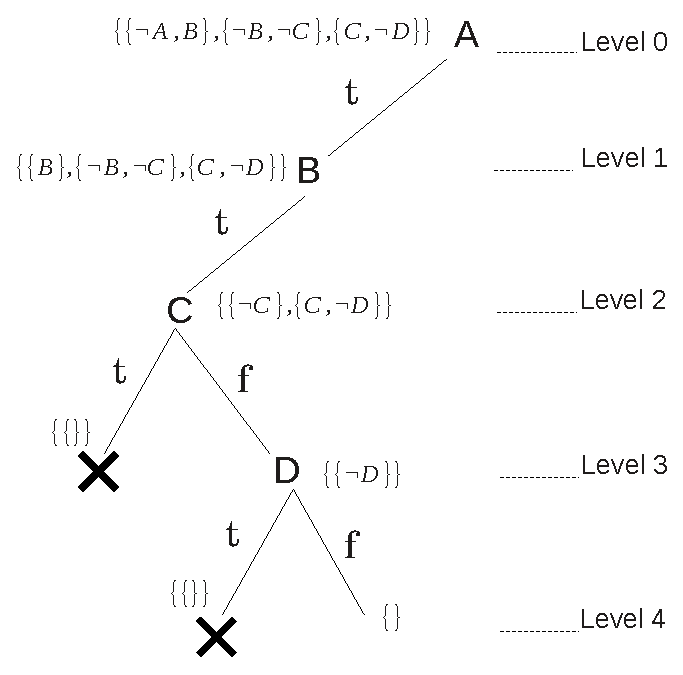
\includegraphics[width=0.5\textwidth]{termination_tree}
	\caption{A termination tree, where each node is labelled by the corresponding CNF. The last node visited during the search is labelled with \{\}. The label X indicates the detection of a contradiction at that node.}
	\label{fig:searchtree}
\end{figure}

Consider the tree of Figure ~\ref{fig:searchtree} and the CNF:
\[\Delta=\{\{\neg A,B\},\{\neg B,\neg C\},\{C,\neg D\}\}.\]
Consider also the node at Level 1, which results from setting variable A to \textbf{true}, and its corresponding CNF:
\[\Delta |A=\{\{B\},\{\neg B,\neg C\},\{C,\neg D\}\}.\]
Algorithm ~\ref{dpll} cannot declare early success or early failure, because the CNF is neither empty, nor contains the empty clause, reason why it keeps searching below Level 1 as shown in Figure \ref{fig:searchtree}. However, we will now show that by using unit resolution, we can declare success success and end the search at Level 1.

The \textit{unit resolution technique} (also called \textit{unit propagation}) is very simple: Before we check tests for success or contradictions, we first collect all unit clauses. Then we assume that the variables which make these clauses unit are set to satisfy the unit clauses. Finally we simplify the CNF and check for success or failure.

To incorporate unit resolution into Algorithm \ref{dpll}, we will introduce a function \textsc{unit-resolution}, which applies to a CNF $\Delta$ and returns two results:
\begin{itemize}
	\item \textbf{I}: a set of literals that are either present as unit clauses in $\Delta$, or were derived from $\Delta$ by unit resolution.
	\item $\Gamma$: a new CNF which results from conditioning $\Delta$ on literals \textbf{I}.
\end{itemize}
For example, if the CNF
\[\Delta=\{\{\neg A,\neg B\},\{B,C\},\{\neg C,D\},\{A\}\},\]
then $\textbf{I}=\{A,\neg B,C,D\}$ and $\Gamma=\{\}$. Moreover, if
\[\Delta=\{\{\neg A,\neg B\},\{B,C\},\{\neg C,D\},\{C\}\},\]
then $\textbf{I}=\{C,D\}$ and $\Gamma=\{\{\neg A,\neg B\}\}$.

\subsubsection{DPLL algorithm}

\begin{algorithm}
$(\textbf{I},\Gamma)=\textsc{unit-resolution}(\Delta)$\\
\uIf{$\Gamma=\{\}$}{
	\bf{return \textbf{I}}.
}
\uElseIf{$\{\}\in \Gamma$}{
	\textbf{return} \textsc{unsatisfiable}
}
\Else{
	choose a literal $L$ in $\Gamma$\\
	\uIf{$\textbf{\textsc{L}}=\textsc{dpll}(\Gamma |L) \neq \textsc{unsatisfiable}$}{
		\textbf{return} \textbf{L} $\cup$ \textbf{I} $\cup$ $\{L\}$	
	}
	\uElseIf{$\textbf{\textsc{L}}=\textsc{dpll}(\Gamma |\neg L) \neq \textsc{unsatisfiable}$}{
		\textbf{return} \textbf{L} $\cup$ \textbf{I} $\cup$ $\{\neg L\}$	
	}
	\Else{
		\textbf{return} \textsc{unsatisfiable}
	}
}
\caption{DPLL(CNF $\Delta$): returns a set of literals or \textsc{unsatisfiable}\label{dpllplus}}
\end{algorithm}    

The DPLL algorithm (Algorithm \ref{dpllplus}) is a refinement of the depth-first-search algorithm. The first change made is that it adds unit resolution in line 1. Also, we no longer assume that variables are examined in the same order as we go down the search tree and we no longer assume that a variable is set to \textbf{true} and then to \textbf{false}. The choice of a literal $L$ on line 7 can have a dramatic impact on the running time of DPLL. This is where inference comes into play when solving a SAT instance with a DPLL based algorithm, heuristics and random factors are commonly used at this point. 

\subsubsection{Chronological backtracking}

When we detect a conflict at level $l$ of the search tree, we have to rewind back to level $l-1$, undoing all assignments done in the process. Then we try another value at level $l-1$, if none remains  to be tried, we then go back further to level $l-2$, and so on. If we ever reach level $0$ and each value there leads to a contradiction, we will know that the CNF is inconsistent. This type of backtracking is called \textit{chronological backtracking}, because the we move back in the same order we got there; one level at a time. 

\subsubsection{Non-Chronological backtracking}

The problem with chronological backtracking, which is the one used in the DPLL algorithm, is that contradictions (when an assignment we have done does not satisfy the CNF) that trigger the backtrack often have valuable information. Such information could lead us to learn new clauses and backtrack more levels than just one, thus saving time in the search. For example, let's say that we have a CNF $\Delta$ with variables $A,B,C,D$. Let's us also say that, because of the clauses in $\Delta$, the CNF will always be inconsistent when $A$ is set to \textbf{true}. Unfortunately, the DPLL algorithm might not realise this beforehand, because it uses unit resolution which is not refutation complete. So the algorithm might only conclude that $A$ set to \textbf{true} will not satisfy $\Delta$ after assigning all possible values to $B,C,D$. If we could detect that $A$ is not part of any solution, we could avoid going any further in that branch of the search tree and learn that information as a new clause (in our example we would learn the clause $\{\neg A\}$ to enforce $A$ to be \textbf{false}). Learning such clauses is called \textit{conflict-driven clause learning} (CDCL) \cite{cdcl1,cdcl2}.

In the next section we will discuss in detail how such new clauses are decided or how can we decide which level to backtrack to after a contradiction is found. Note that adding CDCL features to the DPLL algorithm will not affect its soundness or completeness.

\subsubsection{Clause learning}

When a conflict is detected, the conflict-analysis procedure is used. Such procedure consists of analyzing the conflict structure through \textit{implication graphs} and then learning a clause from it. Let's consider the following CNF:

\begin{equation}\label{row sum}
\Delta = \begin{matrix*}[l]
			1.\{A,B\}\\
		 	2.\{B,C\}\\
		 	3.\{\neg A,\neg X,Y\}\\
		 	4.\{\neg A,X,Z\}\\
		 	5.\{\neg A,\neg Y,Z\}\\
		 	6.\{\neg A,X,\neg Z\}\\
		 	7.\{\neg A,\neg Y,\neg Z\}
		 \end{matrix*}
\end{equation}

The implication graph on Figure \ref{fig:uip} shows a possible search path of a CDCL solver. The nodes of this graph are variable assignments made, with the notation $l/V=v$, where $l$ is a decision level, $V$ a variable and $v$ a truth value. Remember that a variable might be assigned a value in two cases: by a branching decision or by an implication as a result of the propagation process. The directed edges in the graph indicate which assignments implicated other assignments, so an edge from node $\alpha$ to node $\beta$ would mean that the variable assignment in node $\alpha$ implied the assignment shown in node $\beta$. Nodes that do not have any incident edge are decision assignments, because they weren't implied by other assignments. The numeric label on the arcs correspond to the number of the clause that was used for implying that assignment. 

\begin{figure}[h!]
	\centering
		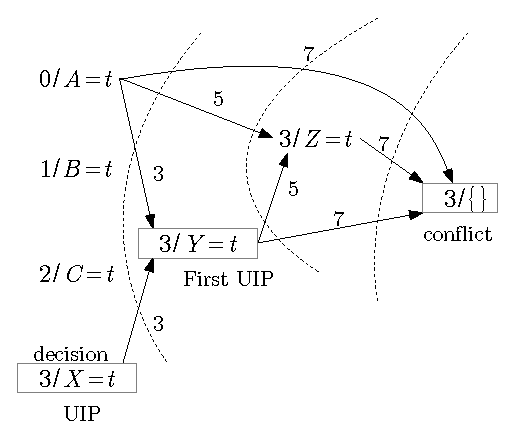
\includegraphics[width=0.7\textwidth]{uip}
	\caption{An implication graph of a conflict}
	\label{fig:uip}
\end{figure}

A \textit{cut} in an implication graph (dashed lines in Figure \ref{fig:uip}) is a set of edges that separate the decision assignments (root nodes) from the contradiction (the leaf node containing $\{\}$). A \textit{conflict set} is a set of variable assignments such that each has an outgoing edge belonging to the same cut, in other words, a conflict set contains enough variable assignments to cause the conflict. Figure \ref{fig:uip} shows three possible cuts for that implication graph, they lead to the conflict sets $\{A=\textbf{true},X=\textbf{true}\}$, $\{A=\textbf{true},Y=\textbf{true}\}$ and $\{A=\textbf{true},Y=\textbf{true},Z=\textbf{true}\}$.

Since there are many possible cuts, and thus conflict sets, we are only interested in choosing the most useful ones. An \textit{asserting} clause \cite{cdcl1} is a clause derived from a conflict set (containing the negation of the assignments in the conflict set) which contains exactly one variable assigned at the level of the conflict. From the previous conflict sets, $\{\neg A,\neg X\}$ and $\{\neg A,\neg Y\}$ are asserting clauses, because only $X$ and $Y$ were decided at the conflict level. 

A refinement to the definition of an asserting clause is the notion of a \textit{unique implication point} (\textit{UIP}) \ref{UIP}. A UIP of a decision level is a variable which was set at that level and that lies in every path from the decision variable at that level to the conflict. For example, the assignments $3/Y=\textbf{true}$ and $3/X=\textbf{true}$ are both UIPs of level 3, and $0/A=\textbf{true}$ is a UIP of level 0. UIPs of a decision level can also be given an order, the first UIP is the one closest to the contradiction. In Figure \ref{fig:uip} the first UIP of level 3 is $3/Y=\textbf{true}$. The \textit{1UIP scheme} \ref{1UIP}, used in modern solvers, learns asserting conflict-driven clauses which have the first UIP of the decision level of the conflict. 

\subsection{Modern CDCL solvers}

Most modern solvers today are CDCL SAT solvers. Given a CNF $\varphi$, a partial assignment of variables $\nu$, Algorithm \ref{cdcl} outlines the general structure of a CDCL SAT solver, where $x$ is a variable, $v$ a truth value and $\beta$ a decision level. We will shortly explain the main functions of this algorithm.

\begin{algorithm}
\KwIn{A CNF $\varphi$ and a variable assignment $\nu$}
\If{\textsc{(UnitPropagation($\varphi$,$\nu$)}=={\bf CONFLICT}\textsc{)}}{
	\bf{return UNSAT}.
}
$dl \leftarrow 0$\\
\While{\textsc{(}{\bf not} \textsc{AllVariablesAssigned($\varphi$,$\nu$))}}{
	\textsc{($x$,$v$)=PickBranchingVariable($\varphi$,$\nu$)}\\
	$dl \leftarrow dl+1$\\
	$\nu \leftarrow \nu$ $\cup$ \{($x$,$v$)\}\\
	\If{\textsc{(UnitPropagation($\varphi$,$\nu$)}=={\bf CONFLICT}\textsc{)}}{
		\textsc{$\beta$=ConflictAnalysis($\varphi$,$\nu$)}\\
		\uIf{\textsc{($\beta < 0$)}}{
			\Return{{\bf UNSAT}}
		}
		\Else{
			\textsc{Backtrack($\varphi$,$\nu$,$\beta$)}\\
			$dl \leftarrow \beta$
		}
	}
}
\Return{\textsc{\textbf{SAT}}}
\caption{Typical CDCL algorithm\label{cdcl}}
\end{algorithm}

\begin{itemize}
	\item \textsc{UnitPropagation} consists of iteratively deducting the truth value of variables. The values are deduced by logical reasoning on $\varphi$ and $\nu$. We already discussed this function in the previous sections.
	\item \textsc{PickBranchingVariable} consists of selecting a variable to assign, and the respective value. Heavily relies in heuristics/random factors to pick variables.
	\item \textsc{ConflictAnalysis} consists of analyzing the most recent contradiction and learning a new clause from it. It returns the decision level to backtrack to (non-chronological backtracking).
	\item \textsc{Backtrack} undoes variable assignments and backtracks to a previous decision level as computed by \textsc{ConflictAnalysis}.
	\item \textsc{AllVariablesAssigned} tests whether all variables have been assigned a truth value.
\end{itemize}


\subsubsection{The two watched literals lazy data structure}

Data structures play a fundamental role in the performance of CDCL SAT solvers. Many improvements have been achieved over the last years, but one of the most noticeable ones is the implementation of the so called \textit{lazy data structures} (lazy because they are not accurate). There are different types of lazy data structures used in modern SAT solvers, they mainly try to address cache performance problems when the solver is performing unit resolution (which adds up to about 70\% of the execution time of a SAT solver \cite{NEEDED}). The two main approaches to implement lazy data structures are the head/tail lists used in Sato \cite{sato} and the two watched literals used in Chaff \cite{chaff}. We will explain the later in detail, as it's widely implemented in most modern CDCL SAT solvers.

\begin{figure}[h!]
	\centering
		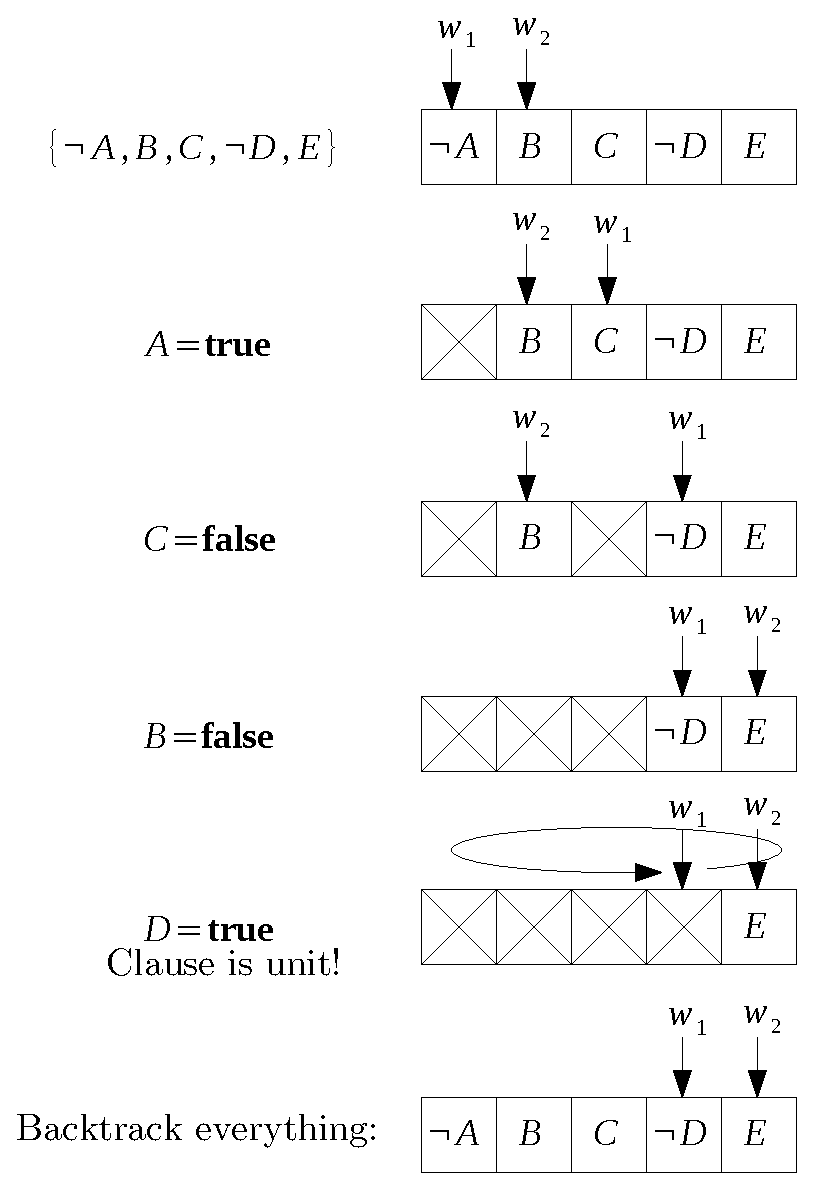
\includegraphics[width=1.0\textwidth]{watchedliterals}
	\caption{Operation of the two watched literal data structure.}
	\label{fig:watched literals}
\end{figure}

Unit propagation is a key function to the speed of a SAT solver. We need fast ways of identifying which clauses become unit when assigning variables. For example, if we have the clause
\[\{\neg A,B,C,\neg D,E\}\]
and the variable assignment
\[A=\textbf{true}, B=\textbf{false}, C=\textbf{false}, E=\textbf{false},\]
we would need to identify somehow that this clause is unit on variable $D$. The two watched literal data structure addresses this problem and makes backtracking very efficient. Instead of trying to keep precise information on the complete state of the clause, the two watched literal strategy only keeps track of two literals in each clause. Such two literals are the watched literals of a clause. Let's take as an example the previous clause, as shown on Figure \ref{fig:watched literals}. This time we will assume that no variable assignments have been done yet and that the two watched literals are $\neg A$ and $B$. Suppose that on the next decision level variable $A$ is assigned as \textbf{true}. We would check the watched literals and realize that this clause might be unit, because now there is only one watched literal which is unassigned and the other doesn't satisfy the clause. Remember that we are only aware of the watched literals and not the rest of them. To check if the clause is really unit, we will attempt to change the first watched literal to an unassigned variable in the clause. We could search to the right and find that literal $B$ is already being watched (the two watched literals must be different), so we keep searching to the right and find that literal $C$ is unassigned, concluding that the clause is not yet unit. Now our two watched literals for this clause are $B$ and $C$. Let's suppose now that propagation gives the value \textbf{false} to variable $C$, then we would again wonder if the clause is unit or not. Searching to the right for another unassigned literal to watch will find literal $\neg D$, so now our two watched literals will be $B$ and $\neg D$. If the next assigned variable is $B=\textbf{false}$, then one watched literal would have to search the clause and find that literal $E$ as available. Finally, if variable $D$ is assigned to \textbf{true}, then we would search the clause for an available literal, but won't find any (after checking all literals). Only now we can declare that this clause is unit, because there is only one unassigned watched literal and the other can't find any unassigned position. Propagation would assign \textbf{true} to variable $E$, because it's the only way to satisfy that clause. If a conflict is found, while propagating across the different variables, we have to undo all variable assignments after the backtracking point, but the key advantage of the two watched literal structure is that no backtracking has to be done to any watched literal reference of any clause. The clear drawback to this advantage is that, as we saw in the previous example, we have to check all literals in the clause before declaring it unit, since we only keep track of two literals at a time.  

\subsubsection{Binary implication lists}

\begin{figure}[h!]
	\centering
		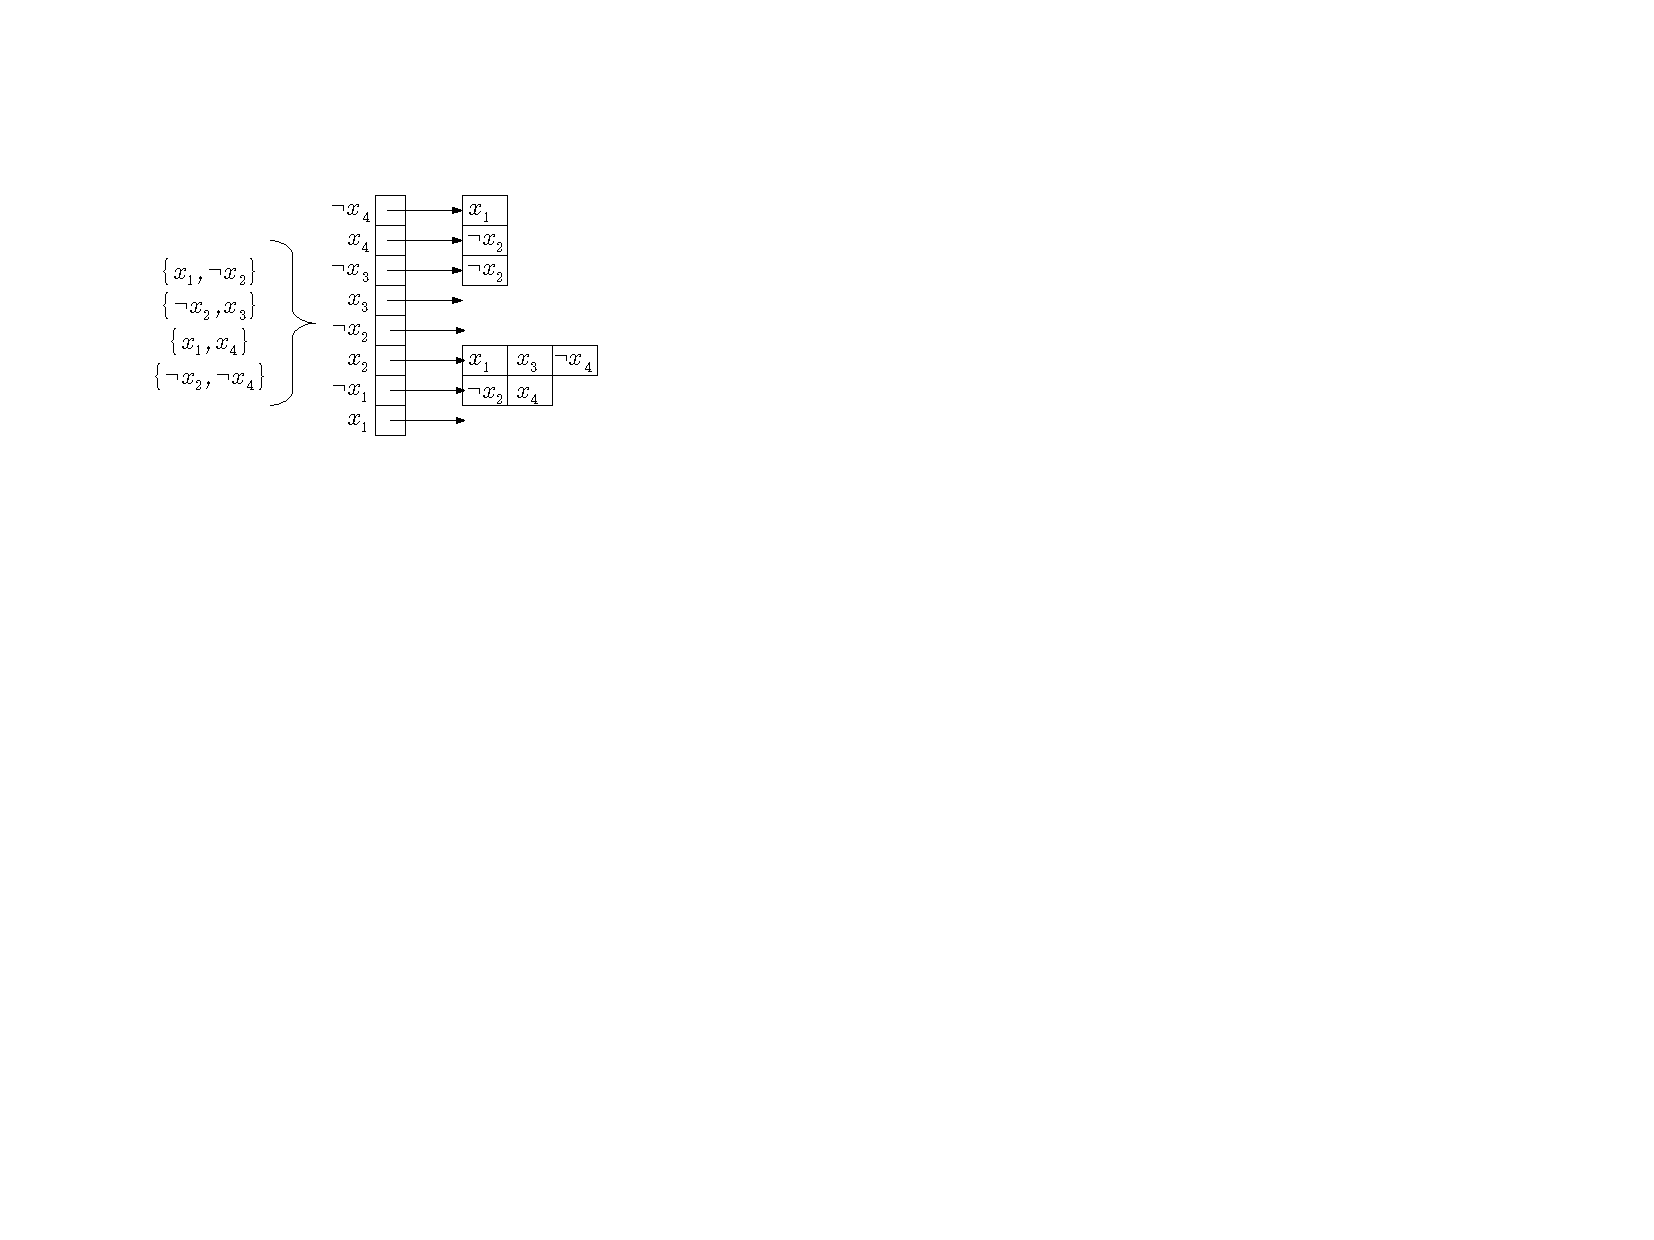
\includegraphics[scale=1]{binary_list}
	\caption{A group of binary clauses and their corresponding binary list.}
	\label{fig:binary list}
\end{figure}

To speed up the propagation of SAT solvers, \textit{Binary clauses}, clauses with two literals, are sometimes stored in special data structures called \textit{binary implication lists}. Binary clauses are frequently used in propagation because they can imply other variable values in just one step. There is also no point on distinguishing two watched literals in these clauses for the simple reason that there are only two literals in them, so knowing when a binary clause is unit becomes trivial. Figure \ref{fig:binary list} represents a set of binary clauses stored in a binary implication list. We have a literal index vector to identify each literal (a variable and its negation), each position of this vector points to a list of literals which are implied by the literal corresponding to the origin of the pointer. Hence, if the $\neg x_{1}$ position in the index vector points to $\neg x_{2}$ and $x_{4}$, this means that if $x_{1}$ were to be \textbf{false}, it would imply that $x_{2}$ must be \textbf{false} and $x_{4}$ \textbf{true}.

\subsection{Parallel SAT solvers}

As mentioned before, some parallel SAT solvers have performed at the top of the last SAT competitions, but even though they all fall into the parallel solvers category, their parallel strategies and implementations vastly differ from each other. We mainly classify parallel SAT solvers into two categories: Portfolio approach solvers and divide-and-conquer solvers.

The main idea behind portfolio approach solvers is the fact that different kinds of sequential solvers will perform differently for different kinds of SAT problems. The portfolio approach is a very straight forward strategy: They run a group of sequential solvers in parallel, each with different heuristic random values and/or different search strategies. The time they take to solve the problem will be the time of the fastest solver in the group of solvers running in parallel. Although all portfolio approach solvers share this same principle, they also have quite different kinds of implementations. We identify in this group the solvers that are pure portfolio approach, the ones that share clauses only logically, and the ones that share clauses physically and logically.

Solvers which are pure portfolio approach have the most simple design. They run completely independent solvers in parallel and wait for one of them to give an answer. Despite their simplicity, the solver ppfolio \cite{ppfolio}, a pure portfolio approach solver, was the winner of the crafted and random categories, and second place in the application category of the 2011 SAT competition of parallel solvers. 

On the other hand, we have more elaborated portfolio approach solvers, which can also share clauses logically between their different solvers. One of the advantages of CDCL solvers is the fact that they can learn new lemmas as they solve a SAT problem. These new lemmas will provide additional information during the solution search, so that the solver doesn't fall into previous fruitless search paths (there are also some drawbacks to adding new lemmas, which are addressed by clause database cleanups). The idea is that different solvers running in parallel can share their learned lemmas so that they all benefit from what other solvers have learned and improve their own search. An example of these kind of solvers is ManySAT \cite{manysat}, which won the 2009 SAT competition in the parallel solver application category. ManySAT has its own sequential state-of-the-art SAT solver and runs different instances of it in parallel, using different VSIDS \cite{vsids} heuristics (branching heuristics) and restart policies for each of it, both of which account for random factors in the solver. The difference with pure portfolio approach solvers, is that ManySAT also shares learned lemmas between solving threads. It is called logical sharing of clauses, because the lemmas are passed as messages between threads and they never share the same physical information in memory. The advantage of logical sharing is that it is easier to implement message passing between threads, than having threads reading and modifying the same memory locations, which often requires locks that could hinder the overall solver performance. One of the best parallel performing solvers, Plingeling \cite{plingeling}, also shares clauses logically. It is a very weak sharing though, since it only shares unit lemmas and it does so through message passing, using a master thread to coordinate messages between worker threads. 

Portfolio approach solvers that share clauses physically have the same strategy as mentioned before, but they share clauses by allowing threads to access the same memory locations, instead of message passing. One solver in this category is SArTagnan \cite{sartagnan}, which shares clauses logically and physically. 

Divide-and-conquer solvers do not try to run different solvers in parallel, they run one solving instance, but try to parallelize the search and divide it between the different threads. A common strategy to divide the search space is to use \textit{guiding paths}. A guiding path is a partial assignment of variables, which restricts the search space of the SAT problem. A solver that divides its search space with guiding paths will assign threads to solve the CNF with the given partial assignment from the guiding path the thread was assigned with. Once a thread finishes searching a guiding path with no success, it can request another to keep searching. MiraXT \cite{miraxt} is a divide-and-conquer SAT solver which uses guiding paths. Moreover, different threads solving different guiding paths also share a common clause database, in which they store their learned lemmas. This is another example of physical clause sharing. 

The work will mainly consist of building a parallel portfolio approach solver, which uses a similar shared clause database system as proposed by MiraXT. The main difference of our work with MiraXT is that we are interested in portfolio approach solving, so we will use the clause database model of MiraXT, but not its divide-and-conquer guiding path strategy. 

\subsubsection{MiraXT}

\begin{figure}[h!]
	\centering
		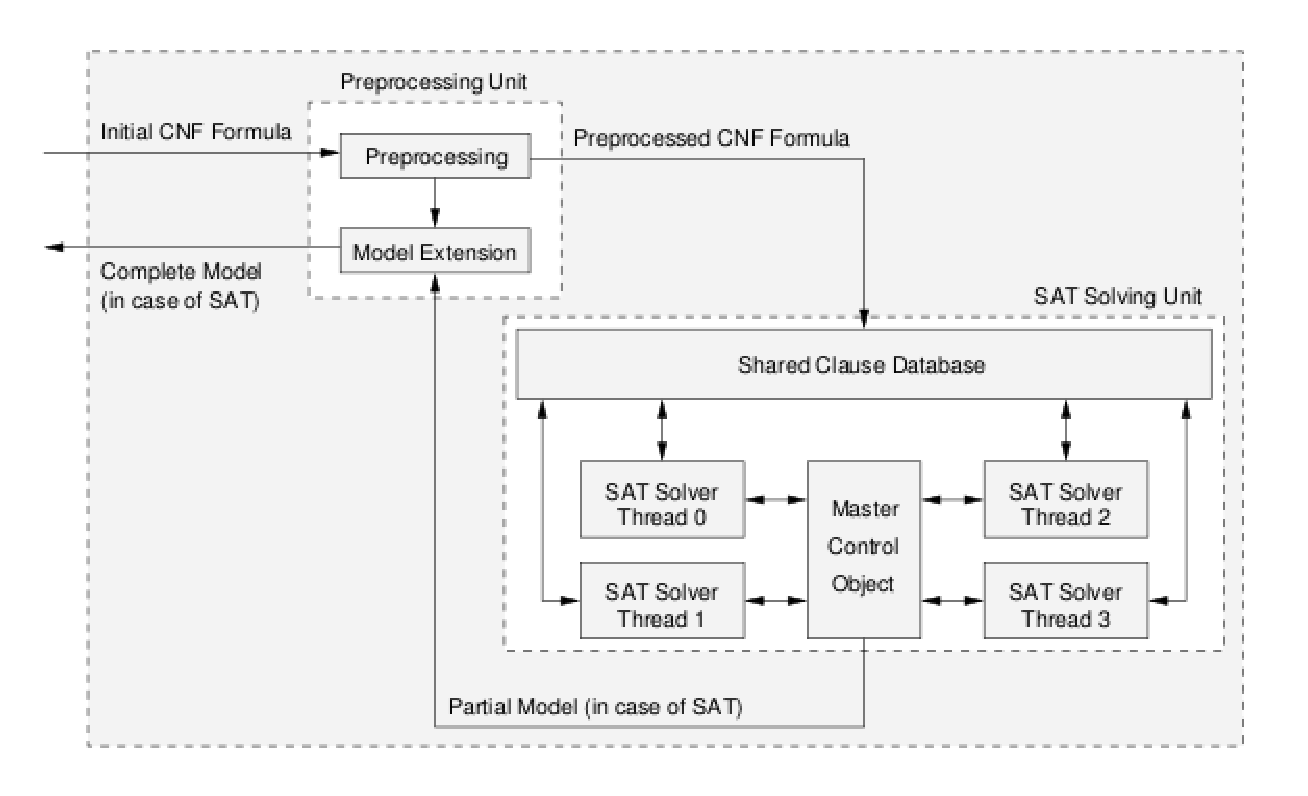
\includegraphics[scale=0.7]{miraxt}
	\caption{Overview of MiraXT design.}
	\label{fig:miraxt overview}
\end{figure}

Figure \ref{fig:miraxt overview} shows the general structure of the MiraXT solver. We are not interested in the \textit{Preprocessing Unit} as it will not be implemented in our solver. The \textit{SAT Solving Unit} is of interest for our work though. The key structure in this design is the \textit{Shared Clause Database}, which is a database of clauses shared among all SAT solving threads. We will also be using this design in our solver, so all threads will be using a common pool of clauses called the Shared Clause Database. The main difference with our design is that we will not have a \textit{Master Control Object} (MCO) structure, which in MiraXT is responsible for the coordination of different threads. The reason for this is that, as we mentioned earlier, MiraXT is a divide-and-conquer solver, so different threads will contribute to one solution and hence will need to be coordinated between each other in this task. On the other hand, our solver will be a portfolio approach one, so different threads will not need to interact with each other directly and no coordination between them is needed.

\begin{figure}[h!]
	\centering
		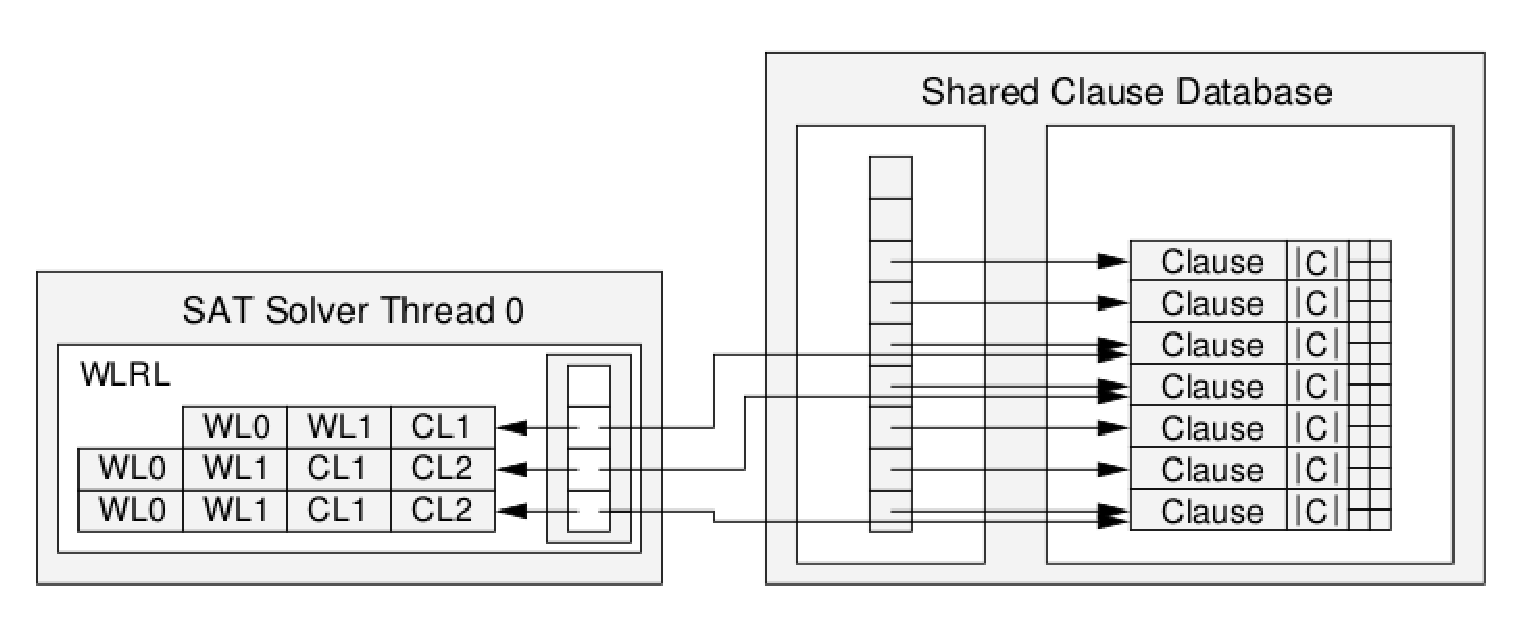
\includegraphics[scale=0.6]{miraxtdatabase}
	\caption{MiraXT shared clause database.}
	\label{fig:miraxt database}
\end{figure}

Regarding the shared clause database, Figure \ref{fig:miraxt database} is a representation of it. Each thread keeps tracks of the two-watched-literals of the clauses it is using, and they also keep two \textit{Cache Literals}, which are used to replace any of the watched literals that need to be updated. If none of the Cache Literals would serve, then they would need to be updated too from the original clauses in the Shared Clause Database. Each clause in each thread has a pointer to the original clause in the Shared Clause Database, so that it knows where to update the Cache Literals from. The Shared Clause Database is read only, so locks are only used when a new clause is inserted, authors mention that lock contention only account for less than $1\%$ of total solving time.

To solve a problem MiraXT will start an initial thread solving the entire problem and depending on whether or not there are idle threads waiting, it will divide the problem into subproblems, with the guiding path technique, and share it with any idle thread. All communication and coordination between threads is done through the MCO with message passing, as shown in Figure \ref{fig:miraxt overview}. 

\section{Cache}

\begin{figure}[h!]
	\centering
		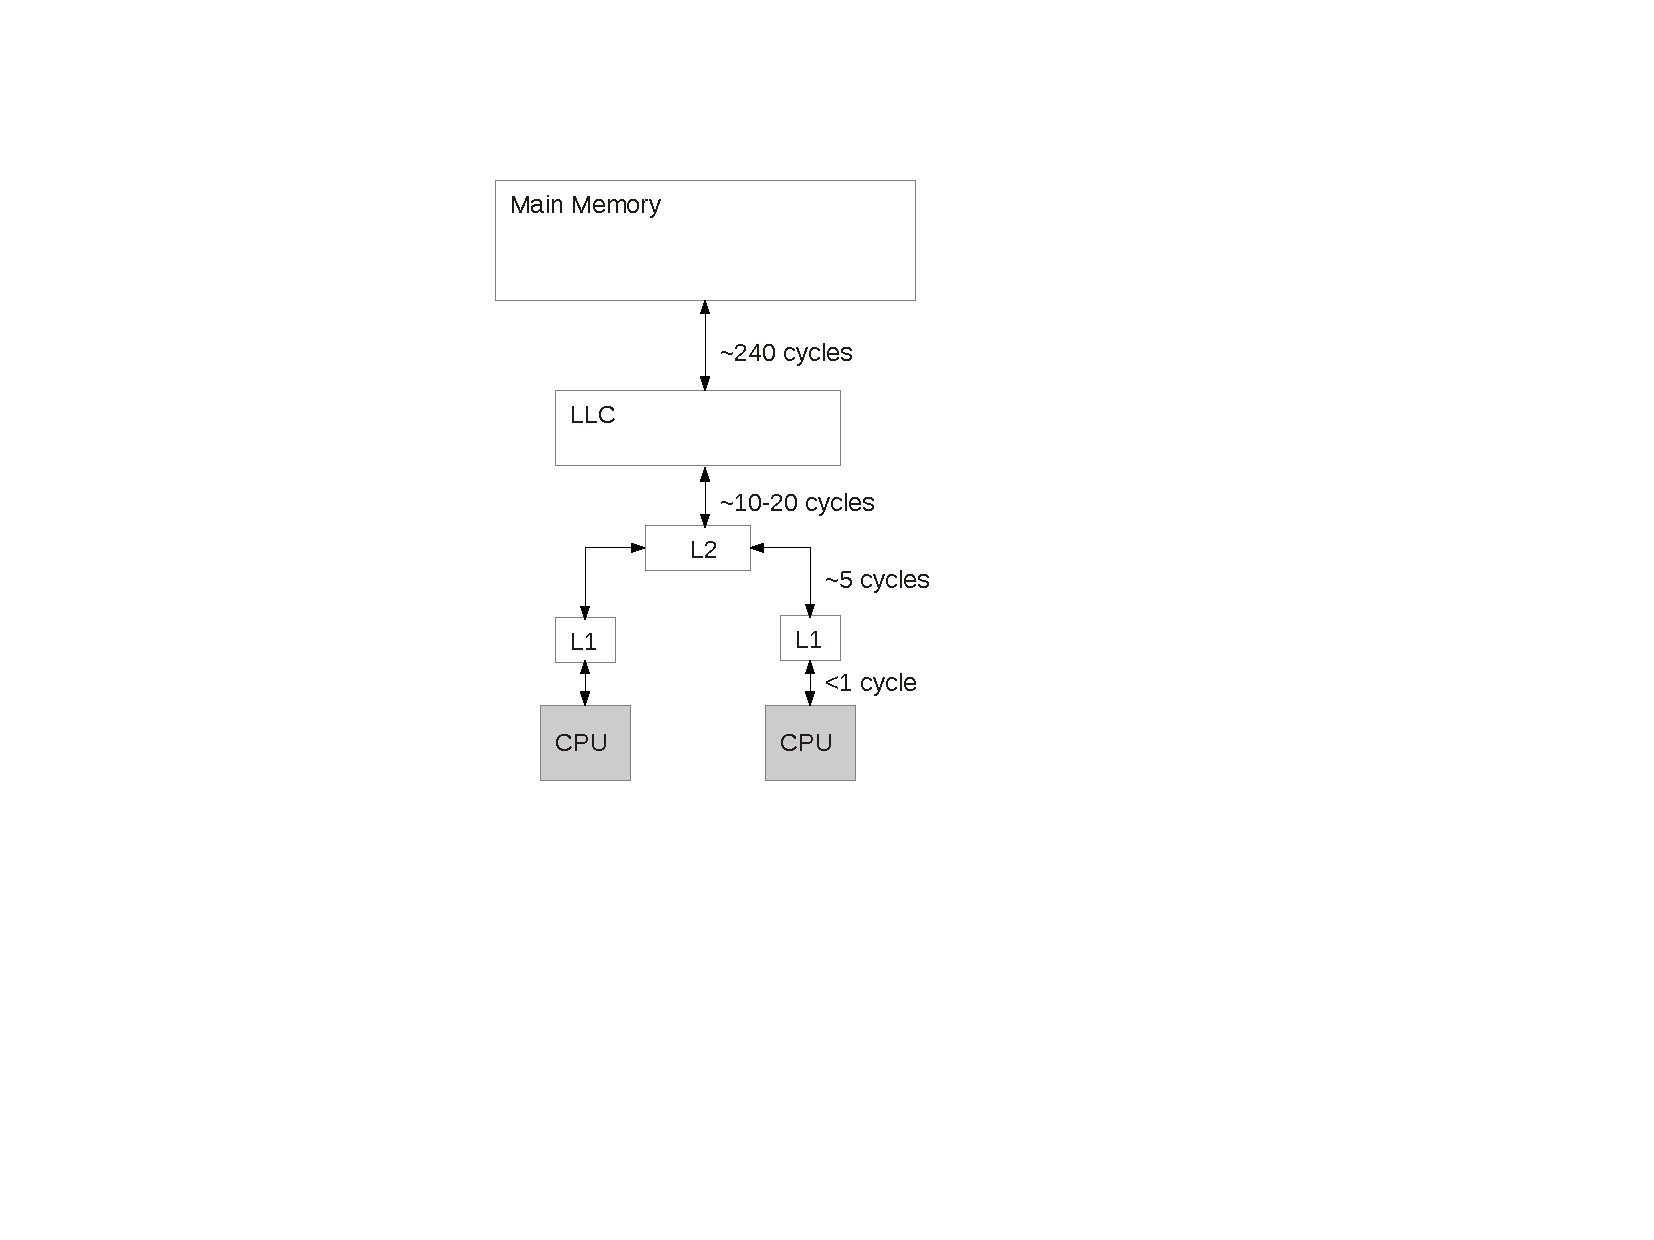
\includegraphics[scale=1]{cache}
	\caption{Typical memory hierarchy of modern computers.}
	\label{fig:cache}
\end{figure}

Computers today usually have three levels of memory cache and a main memory. The processor can have multiple cores in it and cores can run multiple threads in them. The difference between a core and a thread is that cores have separate copies of almost all the hardware resources. The cores can run independently unless they are using the same resource (for example the connection to the outside) at the same time. Threads, on the other hand, share almost all of the processor resources. When a thread, which is running on a core, needs to fetch data, it first tries to look for it in the first level cache (the L1 cache\footnote{There is L1 data cache and also L1 instruction cache, we will be referring to L1 data cache}), if the data is not there, then it tries to find it in the level 2 cache (L2 cache). If the data is still not there, it then tries to fetch it from the level 3 cache (L3 cache) and if that fails too, it goes up to main memory to get the data. If it still isn't in main memory, then it has to retrieve it from the hard disk. We should notice that this hierarchy involves increasing fetch times as we go up. Getting data from the L1 cache is much faster than getting it from L2, and getting data from L2 is much faster than getting it from main memory. The problem with lower level memory is that, because of the technology and costs involved, they are much smaller. So the big picture is that at lower levels we have faster and smaller memories, and at higher levels we have massive and slower memory storages. Figure \ref{fig:cache} is a schematic of today's computer memory hierarchy. To get an idea of the times involved in accessing data from different memory storages, we present the following table of costs associated with hits and misses, for an Intel Pentium M:
\begin{center}
\begin{tabular}{ c | c }
  To where & Cycles \\ \hline
  Register & $\leq 1$ \\
  L1 & ~3 \\ 
  LL & ~14 \\
  Main Memory & ~240 \\
\end{tabular}
\end{center}
 
\subsection{Cache and algorithms} 
 
Another important topic to discuss is how these memory caches operate. When data is requested and it's not found in any of the three caches, it has to be loaded from main memory. Data is not transferred individually, instead, a fixed amount of bytes containing the data (or part of it if it's large) is fetched. This fixed amount of bytes is called a \textit{word} or \textit{cache line}. Intel uses an \textit{inclusive} memory cache protocol, which loads a requested word from main memory into all cache levels. 
Because transferring data from main memory is so costly (compared to any cache level), we would like to transfer the highest amount of useful data from main memory to cache every time. Since the access times to any cache are so little compared to main memory, we will assume the bottleneck of data-fetching performance is main memory. 

\begin{algorithm}
\KwIn{A matrix $M$ of size $m \times n$, which elements are integers}
$sum \leftarrow 0$ \\
\For{$i\leftarrow 0$ \KwTo $m$}{
	\For{$j\leftarrow 0$ \KwTo $n$}{
		$sum=sum+M[i][j]$
	}
}
\Return{sum}
\caption{Row sum of elements\label{matrix row}}
\end{algorithm}

\begin{algorithm}
\KwIn{A matrix $M$ of size $m \times n$, which elements are integers}
$sum \leftarrow 0$ \\
\For{$i\leftarrow 0$ \KwTo $n$}{
	\For{$j\leftarrow 0$ \KwTo $m$}{
		$sum=sum+M[j][i]$
	}
}
\Return{sum}
\caption{Column sum of elements\label{matrix column}}
\end{algorithm}

Data-fetching performance is not only an issue that concerns hardware designers, but also programmers. Depending on how the program is written, the same task (input-output wise) might take much longer if one is not aware about how memory behaves. Since we want the highest amount of useful data in each word transferred, the data structures in which the programmer decides to store data will have a dramatic impact in cache performance. Consider, for example, the following problem: Write a program that sums all elements in a matrix size $m \times n$ of integers. Algorithm \ref{matrix row} and \ref{matrix column} both solve the problem, and apparently with the same level of efficiency, from an algorithmic point of view at least. However, the actual results of both algorithms in practice have a vast difference in total solving time. The following table shows the results for both algorithms implemented in C, for a matrix of size $31000 \times 31000$:
\begin{center}
\begin{tabular}{ c | c }
  Algorithm & Elapsed time (seconds) \\ \hline
  Row sum & 2.8 \\
  Column sum & 28.3 \\ 
\end{tabular}
\end{center}

Figure \ref{fig:matrixmemory} shows a representation of how matrix $M$ could be stored in main memory. As you can see, elements that are in the same row are stored in contiguous memory locations, while elements that are in different columns might be far away from each other. As we mentioned earlier, when an instruction requests data, it will bring a whole word that contains all or some of the data, from main memory to the cache. If we assume that the word size for our example is five integers, then when we fetch element $a$ of the matrix, we will also be fetching the whole row together. If Algorithm \ref{matrix row} is being executed, then after using element $a$, we will need element $b$, but since we already loaded the whole row into cache, there is no need to fetch $b$ from main memory! Same would happen with values $b$, $c$, $d$ and $e$. If, on the other hand, we were executing Algorithm \ref{matrix column}, after using element $a$ we would need to fetch element $f$, but element $f$ was not loaded in cache, so we will need to fetch another word from main memory that contains the $f$ element. Let's suppose now that we only have one level cache and that it can only hold one word at a time (remember cache is much smaller than main memory). Since the cache is full with the word that contains element $a$, we will need to \textit{evict} this word. Evicting a word means pushing it back to main memory and marking the cache line as usable. Once the word containing element $a$ is evicted from cache, we can then proceed to fetch the other cache line containing element $f$. After we have used element $f$, we will then need element $b$ (because we are performing a column sum) and hence produce another eviction and access to main memory. In this simple example, the final count of main memory accesses for Algorithm \ref{matrix row} is two, while for Algorithm \ref{matrix column} is ten. 

\begin{figure}[h!]
	\centering
		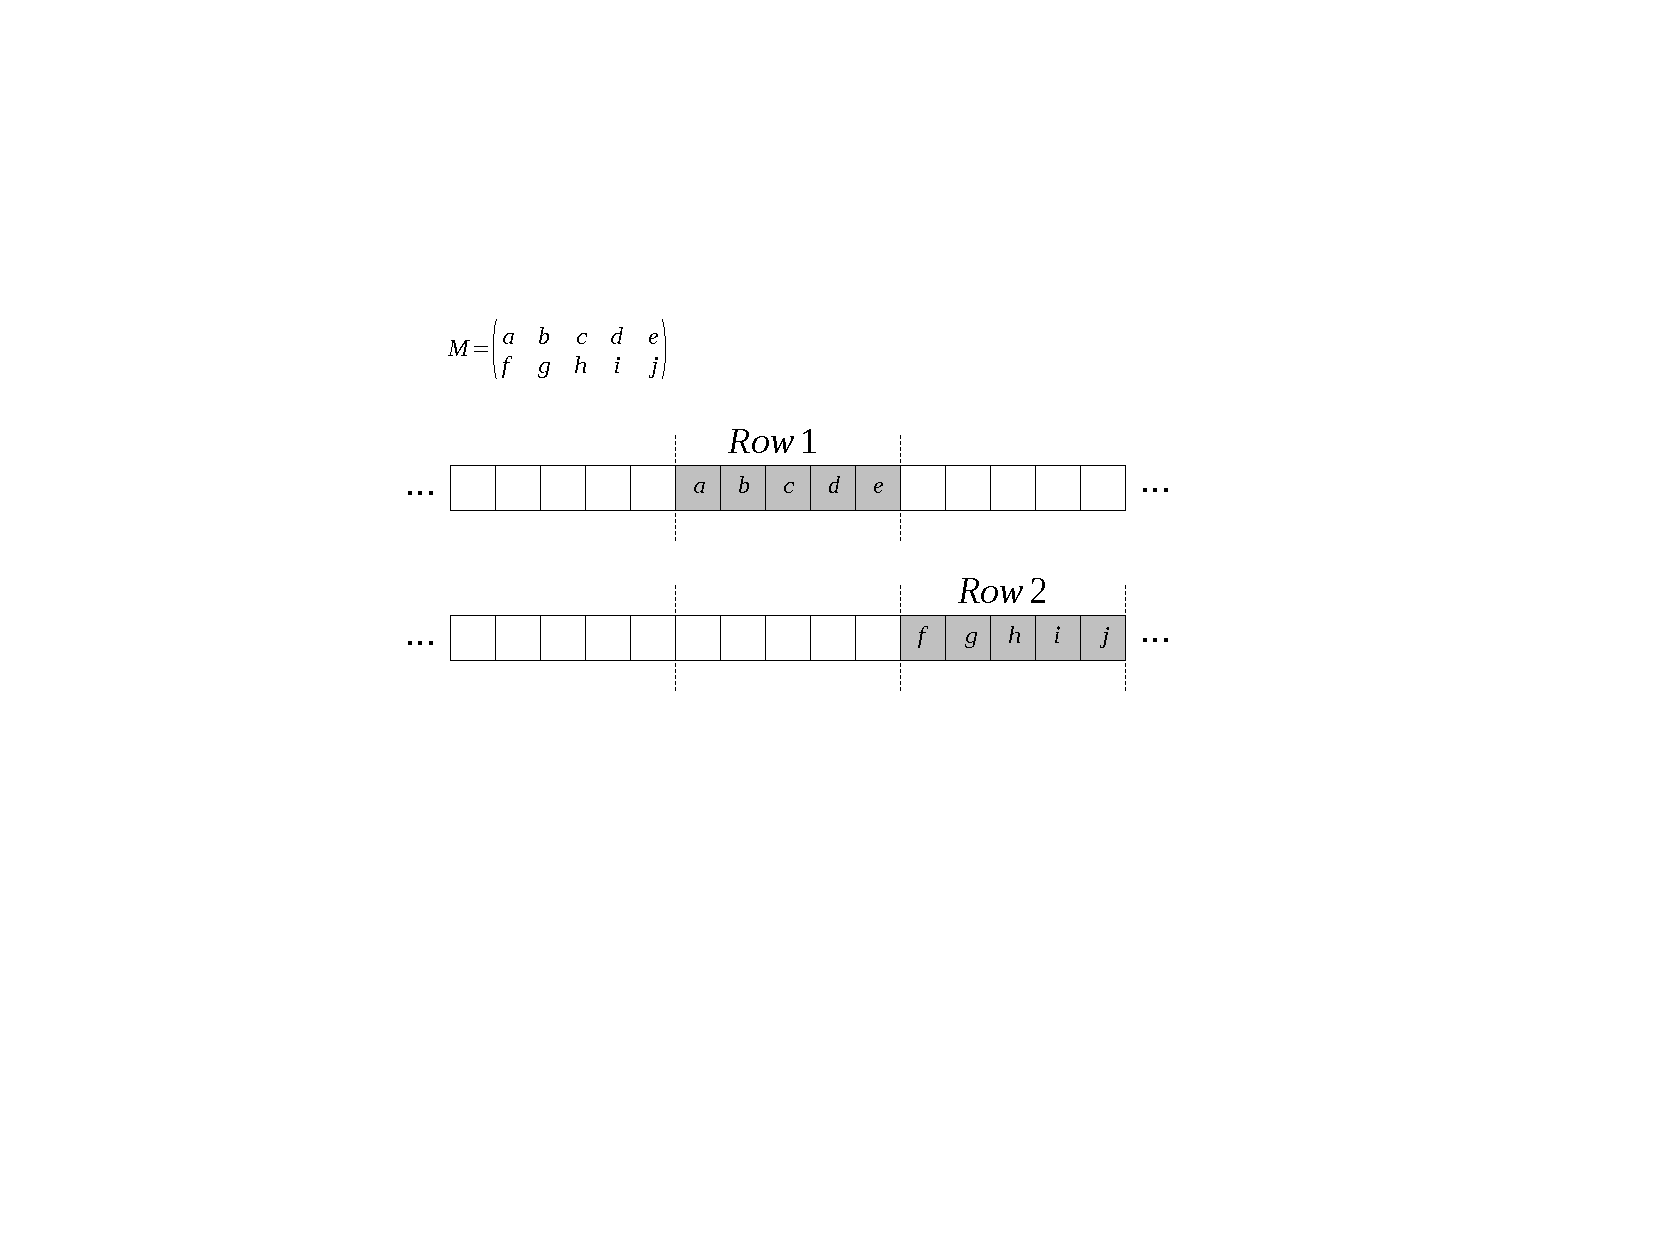
\includegraphics[width=0.7\textwidth]{matrixmemory}
	\caption{A representation of matrix $M$ in main memory.}
	\label{fig:matrixmemory}
\end{figure}

If we generalize our previous example to any matrix size, any word size and any cache size, we will have following formula to calculate the maximum amount of main memory accesses in Algorithm \ref{matrix row}:

\begin{equation}\label{row sum}
t=\left (\frac{n}{w} + 1 \right) \cdot m
\end{equation}

Where $t$ is the number of accesses to main memory, $w$ the word size, $n$ the number of rows of the matrix and $m$ the number of columns. Equation \eqref{row sum} does not take into account the cache size since it will always need to transfer each word containing the rows once. In the big-oh notation, we would have that:

\[ O(t)=\frac{n \cdot m}{w} \]

For Algorithm \ref{matrix column}, the formula to calculate the amount of transfers could be:

\begin{equation}\label{column sum}
t=(n \cdot m) - \left(\left(\frac{c}{w}-1\right)\cdot \left(w-1\right)\cdot n\right),
\end{equation}

assuming that $m\cdot n\gg c$, where $c$ is the cache size.

Equation \eqref{column sum} also depends on other factors though, such as cache eviction policy. For that formula we are assuming a \textit{FIFO} (\textit{First In First Out}) policy, which means that the newest cache line fetched will be evicted when it's necessary. For this case, in big-oh notation, we would have that:

\[ O(t)=n \cdot m \]

So Algorithm \ref{matrix row} will perform better for this problem and is the reason why in practice we see such a big difference between the run time of both algorithms. 

\subsection{Perf: A cache performance tool}

Perf \cite{perf} is a linux tool specialized in collecting and analyzing performance data. The advantage of perf over other performance tools is that it uses special hardware registers dedicated to counting events associated with performance. Other popular tools, such as Valgrind \cite{valgrind}, are software based and emulate the program being monitored to get performance statistics, process that could change the behaviour of the program being studied. The following hardware cache events can be viewed with perf and will be used throughout this work:

\begin{itemize}
\item \textbf{L1-dcache-loads}: The amount of loads done from the L1 data cache to the CPU.
\item \textbf{L1-dcache-load-misses}: The amount of \textit{load misses} from the L1 data cache. A load miss is produced when data is requested from a particular memory level and is not found there, so a load from a higher level in the memory hierarchy is requested.
\item \textbf{LLC-loads}: The amount of loads done from the last level cache (LLC) to the lower level cache (L1 or L2). On modern computers the LLC is usually the L3 cache, which is shared among different cores.
\item \textbf{LLC-load-misses}: The amount of load misses from the LLC.
\end{itemize}

With all the previous information we can draw important results of the cache performance of any program. As an example of the use of perf, we will make a small cache performance analysis of our C program of Algorithm \ref{matrix row} and Algorithm \ref{matrix column}. The perf stats of cache events for Algorithm \ref{matrix row} will yield the following output:

\begin{verbatim}
Performance counter stats for './row_sum':

1,682,744,050 L1-dcache-loads                                     
  132,425,239 L1-dcache-load-misses  #  7.87% of all L1-dcache hits
    4,010,868 LLC-loads              
    3,607,332 LLC-load-misses        # 89.94% of all LL-cache hits

  2.787773717 seconds time elapsed
\end{verbatim}

It should come to our attention that there is a low percentage of L1 cache misses and a high percentage of LL cache misses. The reason why L1 cache misses are so low is because Algorithm \ref{matrix row} sums elements by row, so almost all data that is loaded in L1 is used by the CPU, making the hit percentage very high, as shown in the results. On the contrary, we can also observe that the miss percentage of the LL cache is really high. The reason for this is because when summing elements by rows, we will never need to load the same cache line from the LL cache to L1 (when we load the cache line into L1 we will use all of its elements), hence every time we request data from the LL cache, it will not be there since it's the first time we are requesting that line.

The next output corresponds to the perf stats of the cache performance of Algorithm \ref{matrix column}:

\begin{verbatim}
 Performance counter stats for './column_sum':                                                                                                              
                                                                                                                                                              
 2,652,844,624 L1-dcache-loads                                                                                                        
 2,127,243,131 L1-dcache-load-misses  # 80.19% of all L1-dcache hits                                                                 
 2,037,794,644 LLC-loads                                                                                                              
   506,598,124 LLC-load-misses        # 24.86% of all LL-cache hits                                                                  
                                                                                                                                                              
  27.936225613 seconds time elapsed
\end{verbatim} 

This time the percentage of L1 load misses is very high, this is because we only use one element of the cache line loaded into L1, the next element will be in a different cache line (different columns are not contiguous in memory) so L1 cache hit percentage will be low. On the other hand, the percentage of LL cache misses is much lower than for the row sum algorithm, since we need to load the same cache line more than once, there is a good chance that a line requested will already be in the LL cache. It is important to note that we are mostly interested on what happens in the LL cache, when analyzing cache performance, because every load miss from the LL cache means a load from main memory, which are much more expensive than any other cache load. Under this criteria, one could argue that column sum is better than row sum, because it has a much lower load-miss percentage, but that's why it is also important to take into account the total number of loads and not only percentages. Row sum, despite having a much higher percentage of load-misses, has only a small fraction of the total load-misses on the LL cache that column sum has, hence a much lower number of total loads from main memory.

\subsection{Size does matter}

Aside from the code itself, the amount of data a program handles is also an important factor in cache performance. Let's say we have a square matrix $M$ of size $n$ and that we will perform a fixed number of sums of random elements in the matrix. From an algorithmic point of view, the size of $M$ makes no difference, because the number of sums we will perform is fixed. But again, if we take cache performance into account, the size of matrix $M$ will have a big impact in the time of a program performing this task. Table \ref{tab:matrix_size} shows the different times and cache loads to perform a fixed amount of sums of random elements of different sized matrices. As expected, the number of loads from L1 is kept constant (the small variations are due to other system process running), because we are performing the same amount of operations in all tests. We can also observe that as we increase the size of the matrix, the number of loads from higher level memories also starts increasing. The reason for this is because as the matrix gets bigger, the lower level caches are not big enough to hold all of it, so it uses higher level cache/memory. Only when we start making loads from main memory is when we start noticing differences in time, these results can give us an insight on how expensive loads from main memory are compared to cache ones. The matrix sizes were chosen so that they would only occupy half of each kind of memory level. So the machine has a 32 kB L1 cache, a 262 kB L2 cache, a 8 MB LL cache and 6 GB of main memory.

\begin{table}
\begin{center}
\begin{tabular}{ c | c | c | c | c | c }
  Matrix size & Time (s) & L1 loads & L2 loads & LLC loads & MM Loads \\ \hline
  16 kB 	& 20.8 	& 32673  	& 8  		& $<1$  		& $<1$ 	 \\
  130 kB 	& 20.5 	& 32675  	& 745  		& 8			& $<1$  	 \\ 
  4 MB 		& 27.6	& 32653 	& 1227 		& 910		& 15 	\\
  3000 MB 	& 126.5	& 33278		& 3379		& 2570		& 1446   
\end{tabular}
\caption{Different times and number of memory loads for different size of matrices. The number of loads are in millions of loads.\label{tab:matrix_size}}
\end{center}
\end{table}

%%%%%%%%%%%%%%%%%%%%%%%%%%%%%%%%%%%%%%%%%%%%%%%%%%%%%%%%%%%%%%%%%%%%%%%%%%%%%%%%
% Step 12: Here's the main part of your research project. We can't tell
% you what to write here... that's your job.
%  
%%%%%%%%%%%%%%%%%%%%%%%%%%%%%%%%%%%%%%%%%%%%%%%%%%%%%%%%%%%%%%%%%%%%%%%%%%%%%%%%
\chapter{Important stuff...}\label{chap:contributions}

\section{Cache performance in simple parallel-shared-memory programs}

The main motivation behind this work is our experimental evidence that when threads in different cores share memory, the cache performance improves compared to having threads with its own memory. Our first experiment will be a program that performs simple arithmetic operations on a big matrix. We will have two instances for this experiment. The first will be different threads performing the same arithmetic operations over the same matrix (hence yielding the same result), but every thread will hold its own copy of the big matrix. The second instance will be the same experiment, but this time the different threads will perform the arithmetic operations over the same matrix (regarding physical memory location). For this experience, we will only use read-only operations over the matrix, to keep concurrency problems out of the equation.

To measure cache performance we will use \texttt{perf}. Table \ref{matrix} shows the results of the experiment. Notice that when we share the matrix among threads the cache performance increases significatively. This is because all cores in a single chip share the same LL cache, which has a limited size, so not sharing the matrix means handling a higher volume of data, which hinders cache performance as we saw in the previous chapter. On the other hand, if we share the matrix, then there is a higher chance than the matrix element requested will be found in cache, thus reducing the number of total main memory accesses.

The relation of this experiment to our work is that SAT solvers have a clause database, which would be analogous to the matrix, and different solving threads can also share this clause database, as we do with the matrix. So from this small experiment we can get a hint that sharing the clause database should improve the cache performance of a portfolio approach SAT solver. No doubt that a SAT solver is a much more complex program than the experiment we just did, sharing a clause database is not as a simple as sharing a matrix in this experiment, so it is still not clear if the same results will be obtained when this strategy is applied to a parallel SAT solver.

\section{Cache performance of parallel SAT solvers}

Our first step will be to measure and identify the performance problems that afflict portfolio parallel SAT solvers. The state-of-the-art portfolio approach parallel SAT solver \texttt{plingeling} is one of the best performing parallel solvers to this day. As we mentioned earlier, this solver does not share clauses in any way\footnote{It does share unary clauses through message-passing, but we have deactivated this feature for our experiments.}, so we will measure the performance behaviour as we add more solving threads.

Because portfolio approach SAT solvers implement different search strategies among their solving threads, it is hard to measure the real impact in performance of adding an extra thread. The new thread might implement a successful search strategy, which will make the total solving time improve drastically and hide the negative impact a new thread has in the performance of other threads. This is why we have modified plingeling to make the exact same search in all of its threads. In theory, we would expect the solver to finish at the same time with one thread than with $n$ threads, because all threads are performing the exact same search and thus should finish at the same time. But we know that each solver thread also keeps its own clause database, so basing our reasoning on the previous experiment, we should expect that adding threads will hinder the overall solver performance. So this modified plingeling solver with $n$ threads should perform worse as $n$ grows, assuming that we have enough cores to run $n$ threads and that all cores belong to a same chip. Figure \ref{fig: plingeling performance} shows how the plingeling solver decreases its performance as we add more threads. The decrease in performance is very noticeable and it can even reach 40\%. Our first hypothesis is that this decrease in performance is mostly due to cache issues.

To prove that the problem in scalability lies in cache, we will also perform the experiment on a four chip machine, running each different thread in a different chip. As chips have their own last level cache, we expect the performance decrease to be minimal as we add threads, because different threads will not be sharing cache. Figure \ref{fig:plingeling intel} shows the decrease in performance as we add threads in separate chips. We can observe that the performance decrease in this case is minimal, contrary to the situation where threads are in different cores of a same chip. 

Table \ref{tab:plingeling cache} shows the cache miss percentages as we add more threads to a solver that runs on a single chip. As suggested by our hypothesis, the LLC miss percentage increases dramatically as we add threads, results that explain the decrease in performance of the solver.

\section{A parallel portfolio approach SAT solver with physically shared clause database: AzuDICI}

It is now clear that as we add more data to a SAT solver, we make its performance decrease because of the cache misses involved in handling a bigger volume of data. We will now perform an analysis on how well does sharing data in SAT solvers help reduce the cache misses as we add threads. To be able to do such analysis, we will make a portfolio-approach SAT solver that shares clauses physically, which we named AzuDICI. As we mentioned earlier, there are other solvers which implement physically shared clause databases, but they do not make a detailed analysis of the cache performance of such solvers, which will be the contribution of our experiments with AzuDICI.

\subsection{General outline}

\subsection{Data structures involved}

\subsection{Propagation}

\subsection{Experimental results} 

%%%%%%%%%%%%%%%%%%%%%%%%%%%%%%%%%%%%%%%%%%%%%%%%%%%%%%%%%%%%%%%%%%%%%%%%%%%%%%%%
% Step 13: Add a conclusions chapter
%
% 
%%%%%%%%%%%%%%%%%%%%%%%%%%%%%%%%%%%%%%%%%%%%%%%%%%%%%%%%%%%%%%%%%%%%%%%%%%%%%%%%
\chapter{Conclusions}\label{chap:conclusion}

%%%%%%%%%%%%%%%%%%%%%%%%%%%%%%%%%%%%%%%%%%%%%%%%%%%%%%%%%%%%%%%%%%%%%%%%%%%%%%%%
% Step 14: Work out the bibliography
%
% 
%%%%%%%%%%%%%%%%%%%%%%%%%%%%%%%%%%%%%%%%%%%%%%%%%%%%%%%%%%%%%%%%%%%%%%%%%%%%%%%%
% Tips: 
%
% For named.bst, if I add a~\cite*{} it will add all the references I
% have in the bibliography file (whether they are referenced in the
% document or not)
%%%%%%%%%%%%%%%%%%%%%%%%%%%%%%%%%%%%%%%%%%%%%%%%%%%%%%%%%%%%%%%%%%%%%%%%%%%%%%%%
\bibliographystyle{plain}
\bibliography{biblio}

\end{document}
